\begin{Exercise}[title=Slalom entre des cheminées :Star Wars]
	\begin{center}
		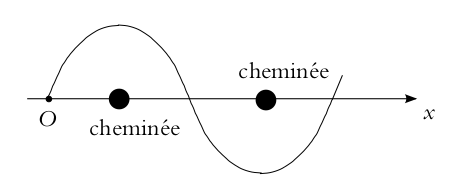
\includegraphics[width=0.5\linewidth]{../fig/starwars.png}
	\end{center}
	Dans cet épisode de la Guerre des Étoiles, on peut assister à une course poursuite de « speeder » entre des cheminées d’usine. On suppose que le véhicule suit une trajectoire sinusoïdale de slalom entre les cheminées alignées selon l’axe Ox. Elles sont espacées d’une distance L = 200 m.
	\Question Le véhicule conserve une vitesse v 0 constante selon Ox. Il met un temps t t = 12 s pour revenir sur l’axe après la sixième cheminée. En déduire la vitesse $v_0$ . Effectuer l’application numérique.
	\Question Déterminer l’amplitude de la sinusoïde pour que l’accélération reste inférieure à 10g en 	valeur absolue, avec$ g = $\SI{9, 8}{\m\per\s^2} . Que penser des valeurs obtenues ?
	\Question (*) Dans quel épisode à lieu cette course poursuite
\end{Exercise}
\begin{Answer}
  \Question $y = a \cos(2\pi v_0 t /L)$ avec $v_0=6L/t_1 =$ \SI{100}{\m\per\s}.
	\Question on veux $a \left(\frac{2\pi v_0}{L}\right)^2 \leq 10g$ alors  $a =9.9$ m ,il faut être un Jedi pour réussir une telle manœuvre
	\Question Star Wars 2, l'attaque des clones
\end{Answer}
